\documentclass[10pt,a4paper,twocolumn]{article}
\usepackage[margin=0.5in]{geometry}
\usepackage{graphicx}
\usepackage{amsmath}
\usepackage{amssymb}
\usepackage{caption}
\usepackage{subcaption}
\usepackage{float}
\usepackage{booktabs}
\usepackage{microtype}
\captionsetup{font=footnotesize,skip=1pt}
\setlength{\parskip}{0.15em}
\setlength{\parindent}{0pt}
\setlength{\textfloatsep}{4pt}
\setlength{\intextsep}{3pt}
\setlength{\abovecaptionskip}{1pt}
\setlength{\belowcaptionskip}{0pt}
\setlength{\columnsep}{18pt}

\begin{document}

\twocolumn[{\centering
  \vspace{-1.5em}
  {\Large\bfseries DSAI 490 -- Assignment 1\\[2pt]
   Representation Learning with Autoencoders (AE \& $\beta$-VAE) on Medical MNIST}\par
  \vspace{0.3em}
  Amr Yasser\par
  \vspace{0.8em}
}]

\section{Introduction and dataset}
This work implements and compares a convolutional Autoencoder (AE) and a convolutional $\beta$-Variational Autoencoder ($\beta$-VAE) on the Medical MNIST dataset, which contains six classes of $64{\times}64$ grayscale medical images (AbdomenCT, BreastMRI, CXR, ChestCT, Hand, HeadCT). Data is split $80/10/10$ train/validation/test and streamed through a \texttt{tf.data} pipeline (JPEG decoding, resize, $[0,1]$ scaling, shuffle, batch, prefetch). Both models train for 30 epochs with Adam ($10^{-3}$) and batch size 128 on a single Kaggle GPU. The full codebase, trained weights, and all figures are reproduced by a single Jupyter notebook.

\section{Model architectures}
\textbf{Autoencoder.} A convolutional encoder with three \texttt{Conv2D + MaxPooling2D} blocks (filters $32{\to}16{\to}16$) compresses $64{\times}64{\times}1$ inputs to an $8{\times}8{\times}16$ feature map (1024 latent dimensions). The decoder is a symmetric stack of three \texttt{Conv2DTranspose} layers with stride 2, followed by a final $3{\times}3$ sigmoid \texttt{Conv2D}. Loss is pixelwise binary cross-entropy.

\textbf{$\beta$-Variational Autoencoder.} The encoder uses three strided \texttt{Conv2D} layers ($32{\to}64{\to}64$), a 128-unit dense layer, and two parallel dense heads producing $\boldsymbol{\mu}, \log\boldsymbol{\sigma}^2 \in \mathbb{R}^{16}$. The reparameterisation trick $\mathbf{z} = \boldsymbol{\mu} + \boldsymbol{\sigma} \odot \boldsymbol{\epsilon}$, $\boldsymbol{\epsilon} \sim \mathcal{N}(\mathbf{0}, \mathbf{I})$, yields a differentiable sample that the decoder (dense $\to$ reshape $\to$ three \texttt{Conv2DTranspose} $\to$ sigmoid) reconstructs. The objective is the evidence lower bound with a scalar Kullback--Leibler weight:
\[
  \mathcal{L} = \underbrace{\mathbb{E}_{q}\!\left[\mathrm{BCE}(x, \hat x)\right]}_{\text{reconstruction}} + \beta \cdot \underbrace{\mathrm{KL}\!\left(q(z\mid x)\,\|\,\mathcal{N}(\mathbf{0}, \mathbf{I})\right)}_{\text{regulariser}},
\]
with KL computed in closed form. We set $\beta = 0.25$: a pilot run at $\beta = 1$ exhibited partial posterior collapse (KL $\approx 27$ nats) and severely blurred reconstructions, a known failure mode on datasets where BCE summed over pixels dominates the KL term. Down-weighting KL recovers encoding capacity; lowering $\beta$ \emph{raises} KL (observed $\approx 43$ nats) because the encoder is allowed to move further from the prior.

\textbf{Key difference.} The AE has a deterministic 1024-dim code with no prior regularisation and is optimised only for reconstruction. The $\beta$-VAE has a probabilistic 16-dim code actively pulled toward a unit-Gaussian prior. The VAE therefore trades code capacity and class-wise separability for a continuous, sampleable latent --- the price of a real generative model.

\section{Results}

\begin{figure}[H]
  \centering
  \begin{subfigure}{0.32\linewidth}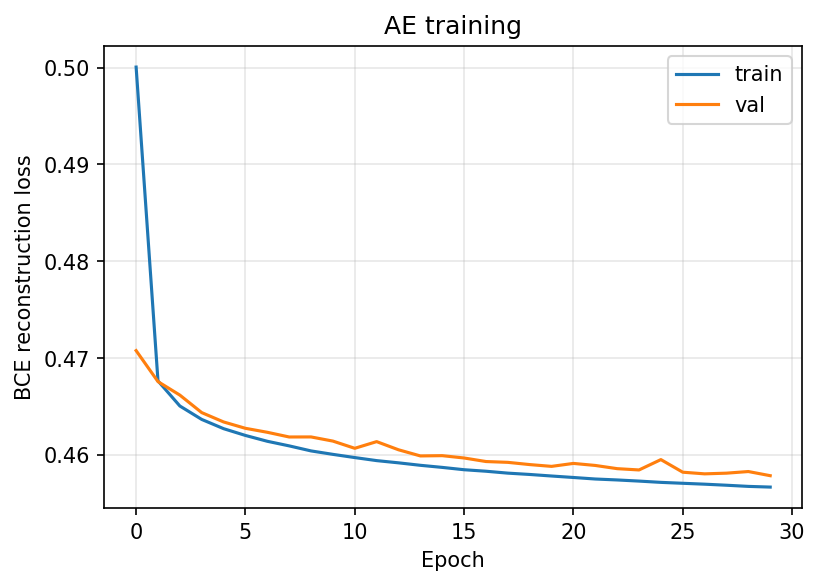
\includegraphics[width=\linewidth]{../figures/02_ae_loss.png}\caption{AE (BCE)}\end{subfigure}\hfill
  \begin{subfigure}{0.66\linewidth}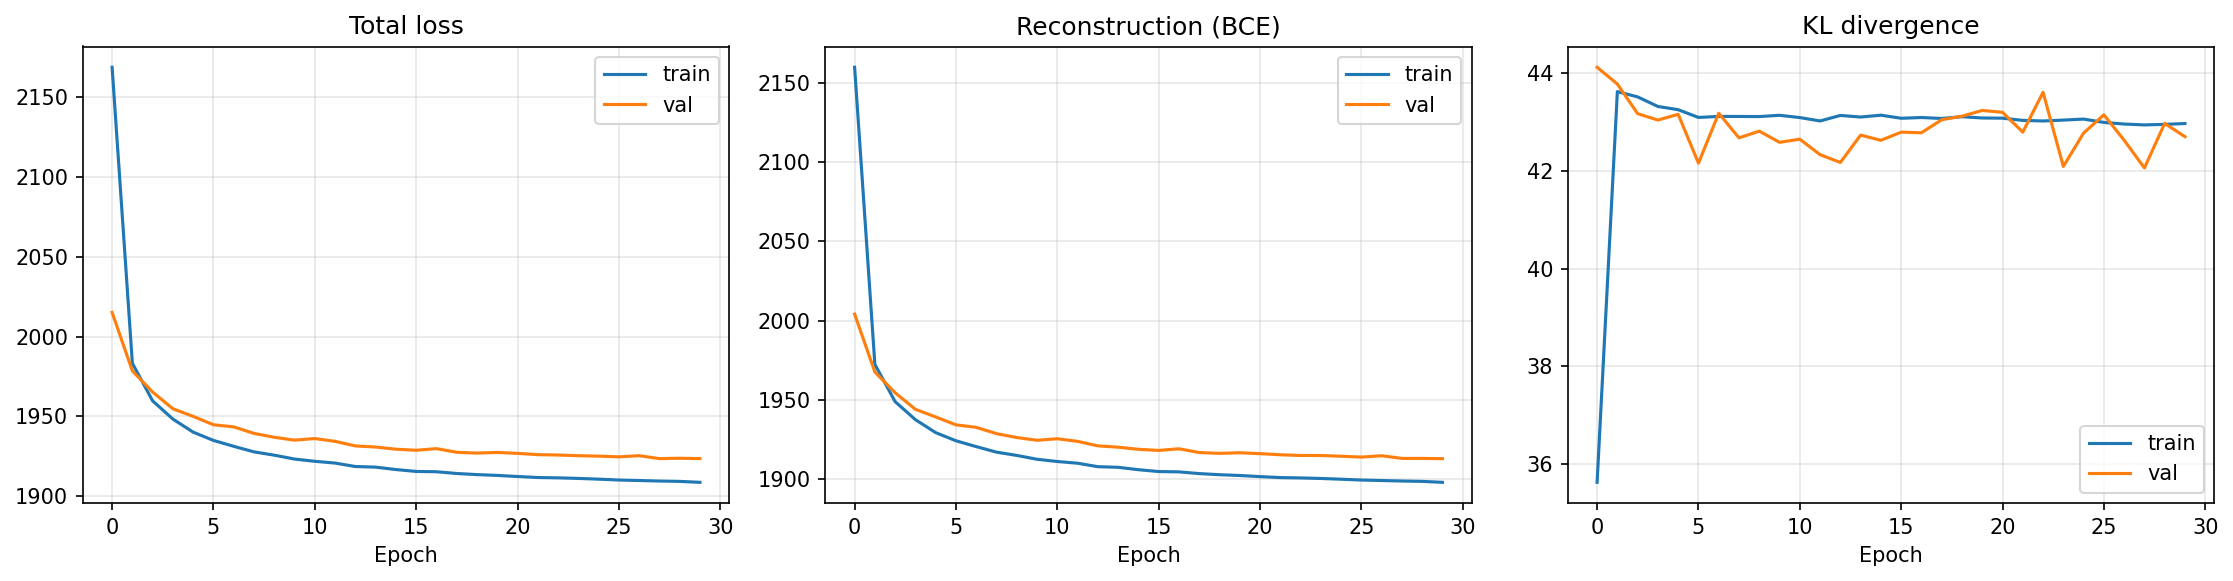
\includegraphics[width=\linewidth]{../figures/03_vae_loss.png}\caption{VAE: total / reconstruction (BCE) / KL}\end{subfigure}
  \caption{Training dynamics. AE BCE drops from $0.50$ to $0.46$ and plateaus after $\sim$20 epochs. The VAE reconstruction term drops from $\sim$2160 to $\sim$1900, while KL rises from its initialisation and stabilises at $\sim$43 nats --- the encoder learning to carry information rather than collapsing to the prior.}
  \label{fig:loss}
\end{figure}

\textbf{Reconstruction (Fig.~\ref{fig:recon}).} Table~\ref{tab:metrics} shows the AE achieves lower test pixel error than the $\beta$-VAE, as expected: the AE has 1024 unregularised dimensions versus 16 regularised ones and is optimised for exactly this objective. Both models reproduce coarse anatomy faithfully (hand fingers, chest cavity, skull silhouette); fine texture --- trabecular bone in the Hand, parenchymal detail in HeadCT, peritoneal structure in AbdomenCT --- is partially lost. The VAE output is visibly smoother, the canonical ``VAE blur'' driven by the 16-dim KL-regularised code and the Gaussian output likelihood.

\begin{figure}[H]
  \centering
  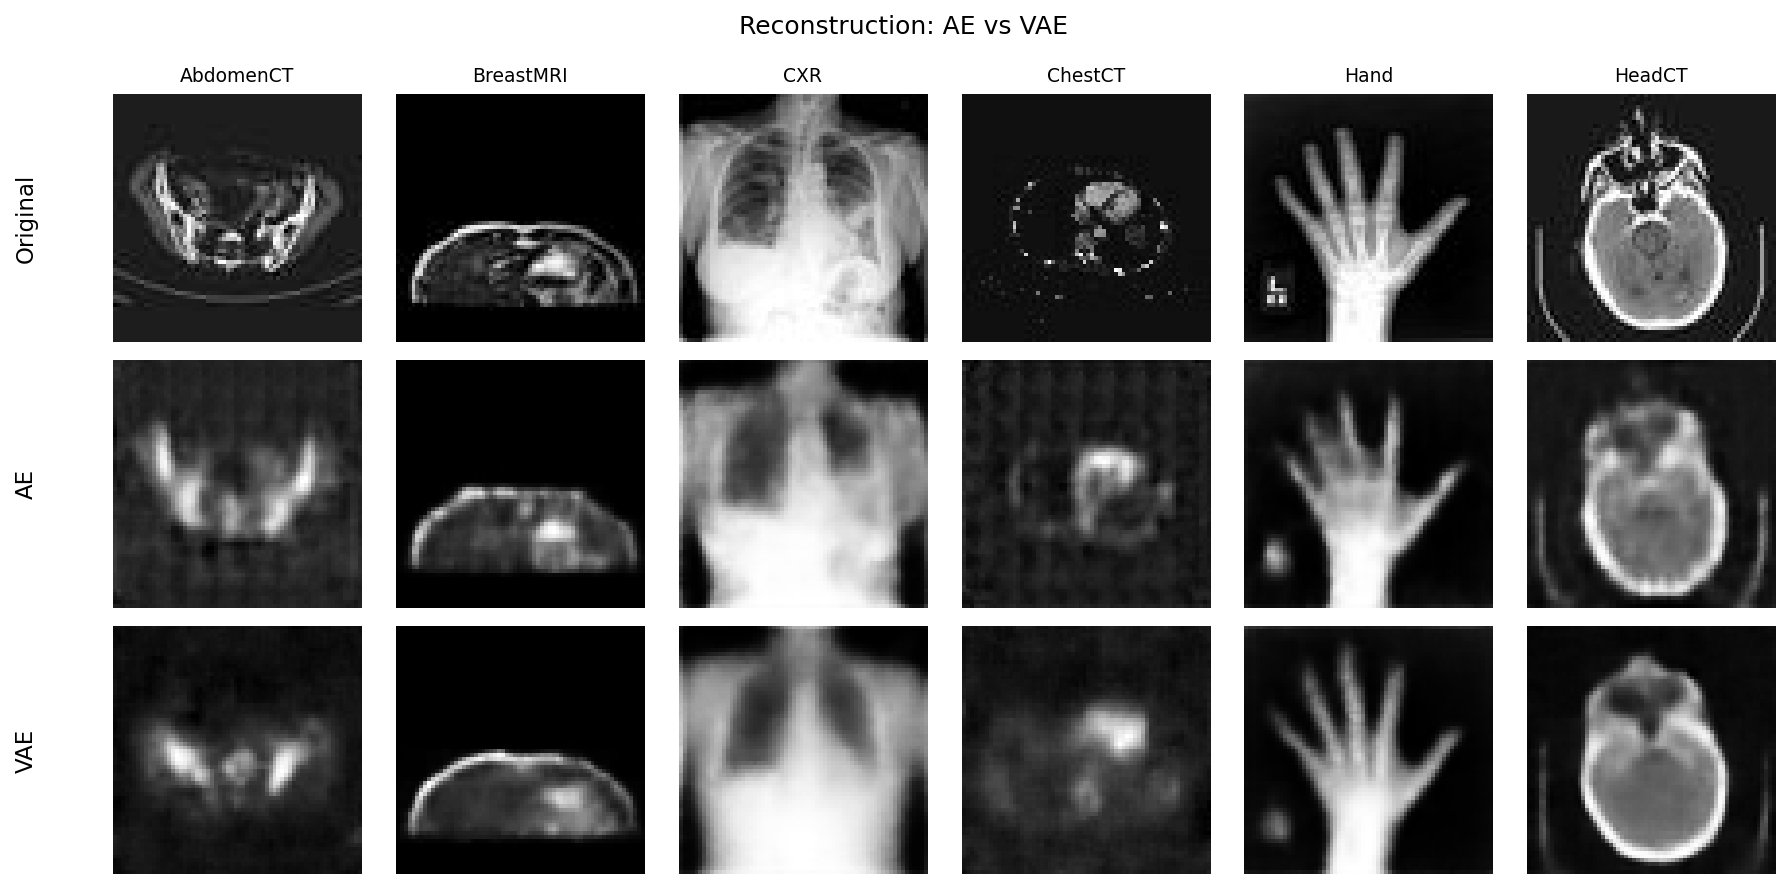
\includegraphics[width=\linewidth]{../figures/04_reconstruction_comparison.png}
  \caption{Reconstruction, one test example per class. Top: original. Middle: AE. Bottom: $\beta$-VAE. Both preserve global structure; both soften high-frequency texture.}
  \label{fig:recon}
\end{figure}

\begin{table}[H]
  \centering\footnotesize
  \begin{tabular}{lcc}
    \toprule
                 & \textbf{Test MSE} & \textbf{Test MAE} \\
    \midrule
    AE           & $0.00429$ & $0.0355$ \\
    $\beta$-VAE  & $0.00699$ & $0.0449$ \\
    \bottomrule
  \end{tabular}
  \caption{Pixel-wise reconstruction error on the held-out test set.}
  \label{tab:metrics}
\end{table}

\begin{figure}[H]
  \centering
  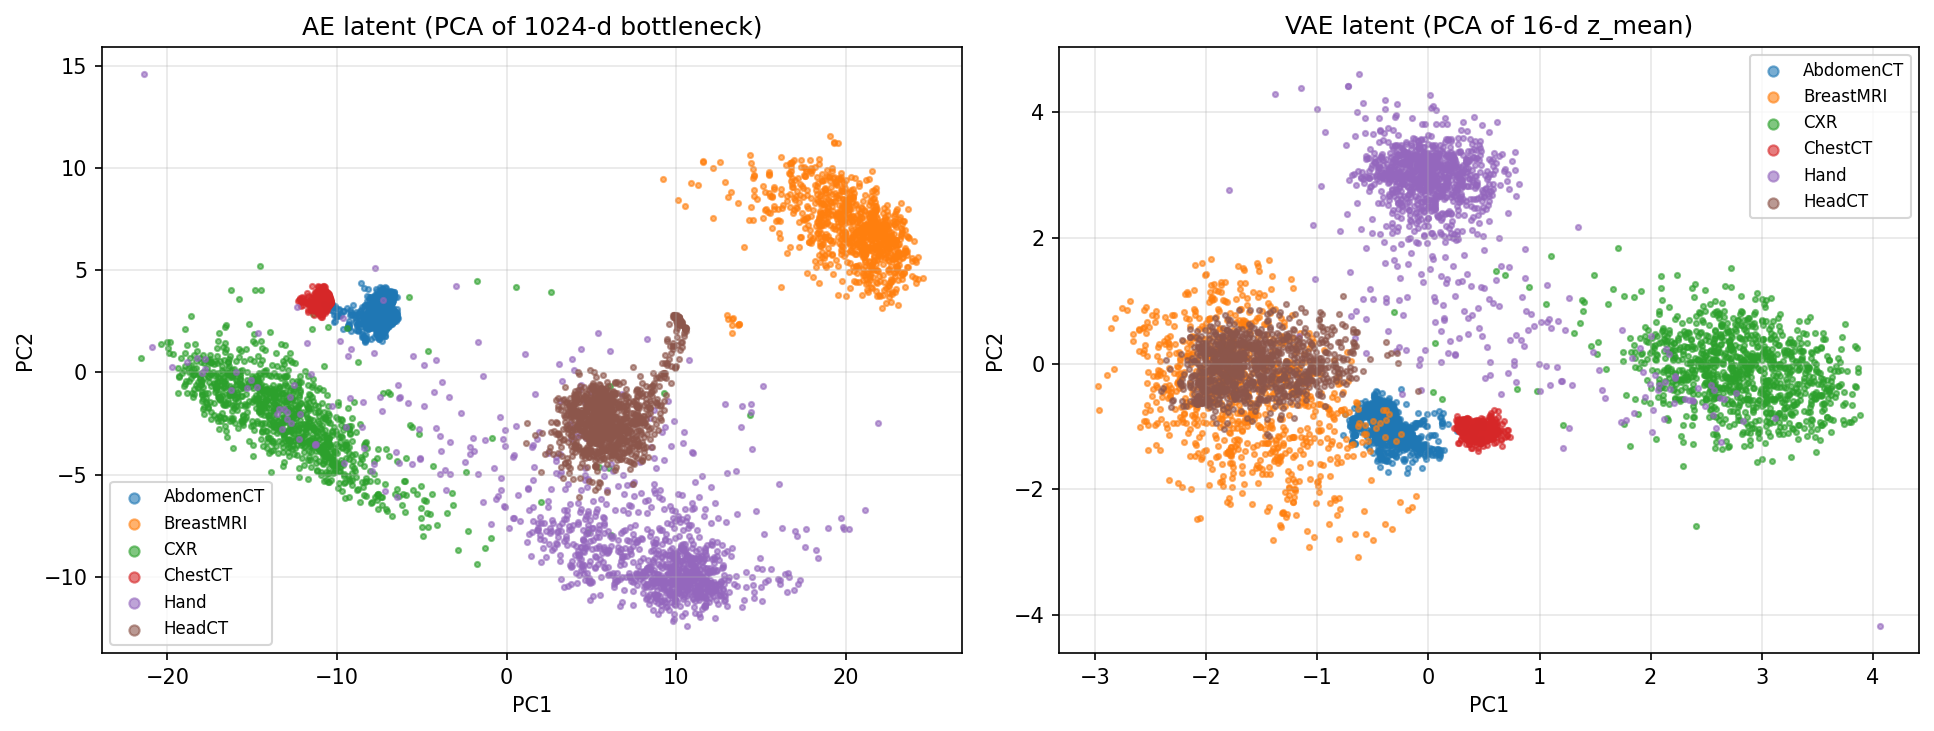
\includegraphics[width=\linewidth]{../figures/05_latent_space_pca.png}
  \caption{2D PCA of test-set latents. AE (left): 1024-dim deterministic bottleneck yields tight, well-separated class clusters. $\beta$-VAE (right): 16-dim $\boldsymbol{\mu}$-space is compact and centered near the origin (by prior regularisation) with visible class structure but more inter-class overlap.}
  \label{fig:latent}
\end{figure}

\textbf{Latent space (Fig.~\ref{fig:latent}).} The AE bottleneck places BreastMRI, Hand, and the CT group in clearly distinct regions; this is precisely the structure a downstream classifier wants. The VAE $\boldsymbol{\mu}$-space is more compressed and more overlapping --- an unavoidable consequence of KL regularisation pulling every posterior toward the same prior. The VAE latent is nonetheless densely and continuously populated near the origin, which is what makes the \emph{prior} distribution a meaningful generative target.

\begin{figure}[H]
  \centering
  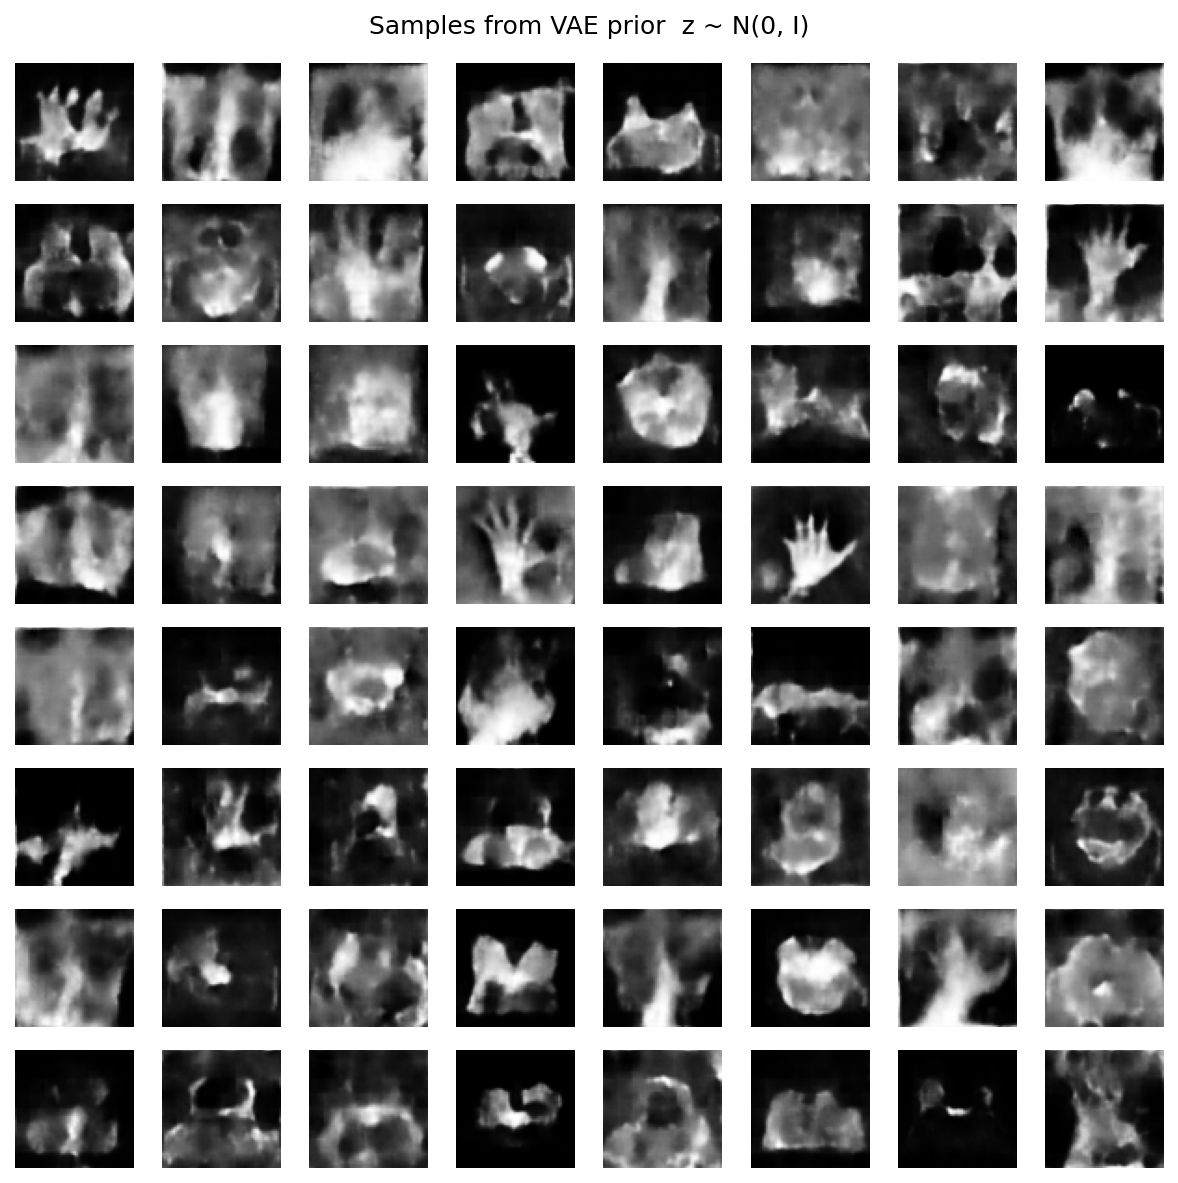
\includegraphics[width=\linewidth]{../figures/06_vae_generated_samples.png}
  \caption{$64$ samples $\hat x = \mathrm{dec}(z),\ z \sim \mathcal{N}(0, I)$. Several samples are class-identifiable (hands in rows~2 and~4, chest-cavity silhouettes in rows~1 and~5); others are class-ambiguous blends typical of a small convolutional VAE with a unit-Gaussian prior.}
  \label{fig:gen}
\end{figure}

\begin{figure}[H]
  \centering
  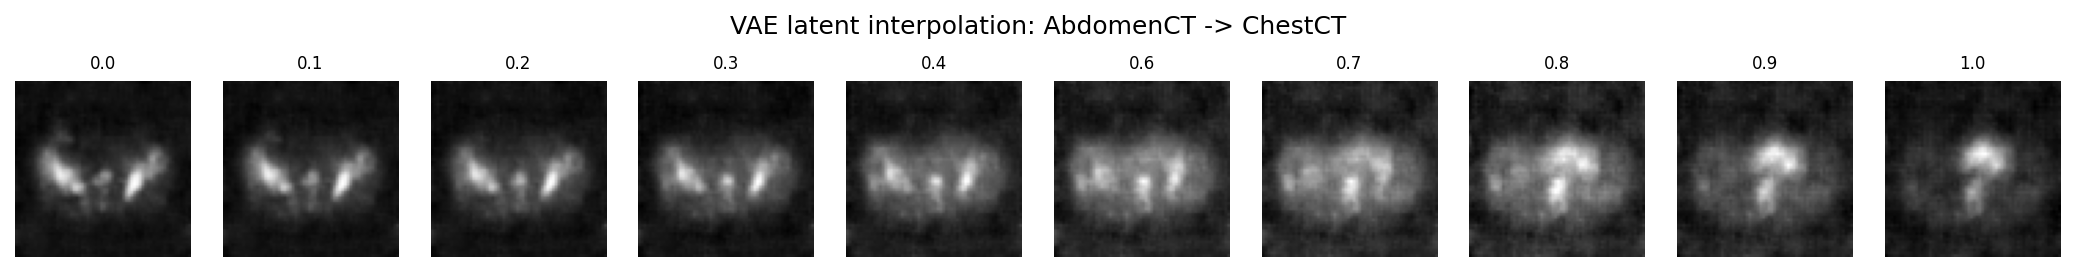
\includegraphics[width=\linewidth]{../figures/07_vae_interpolation.png}
  \caption{Linear interpolation in $\boldsymbol{\mu}$-space between an AbdomenCT and a ChestCT encoding. Smooth pixel-level transitions (no discrete jumps) indicate a continuous latent manifold, even though the intermediate frames remain visually ambiguous on this dataset.}
  \label{fig:interp}
\end{figure}

\textbf{Sample generation and interpolation.} Figure~\ref{fig:gen} shows that the $\beta$-VAE has learned a generative distribution: hands and chest silhouettes emerge recurrently across the grid, confirming class structure in the prior. Samples are blurry --- a property bounded by the Gaussian likelihood and small latent, not by training length. Richer priors (VQ-VAE, diffusion) are required for sharp medical-image synthesis at substantially higher cost. Figure~\ref{fig:interp} confirms that the latent manifold is smooth: no discontinuities appear along the path, a prerequisite for using the latent for semantic editing.

\begin{figure}[H]
  \centering
  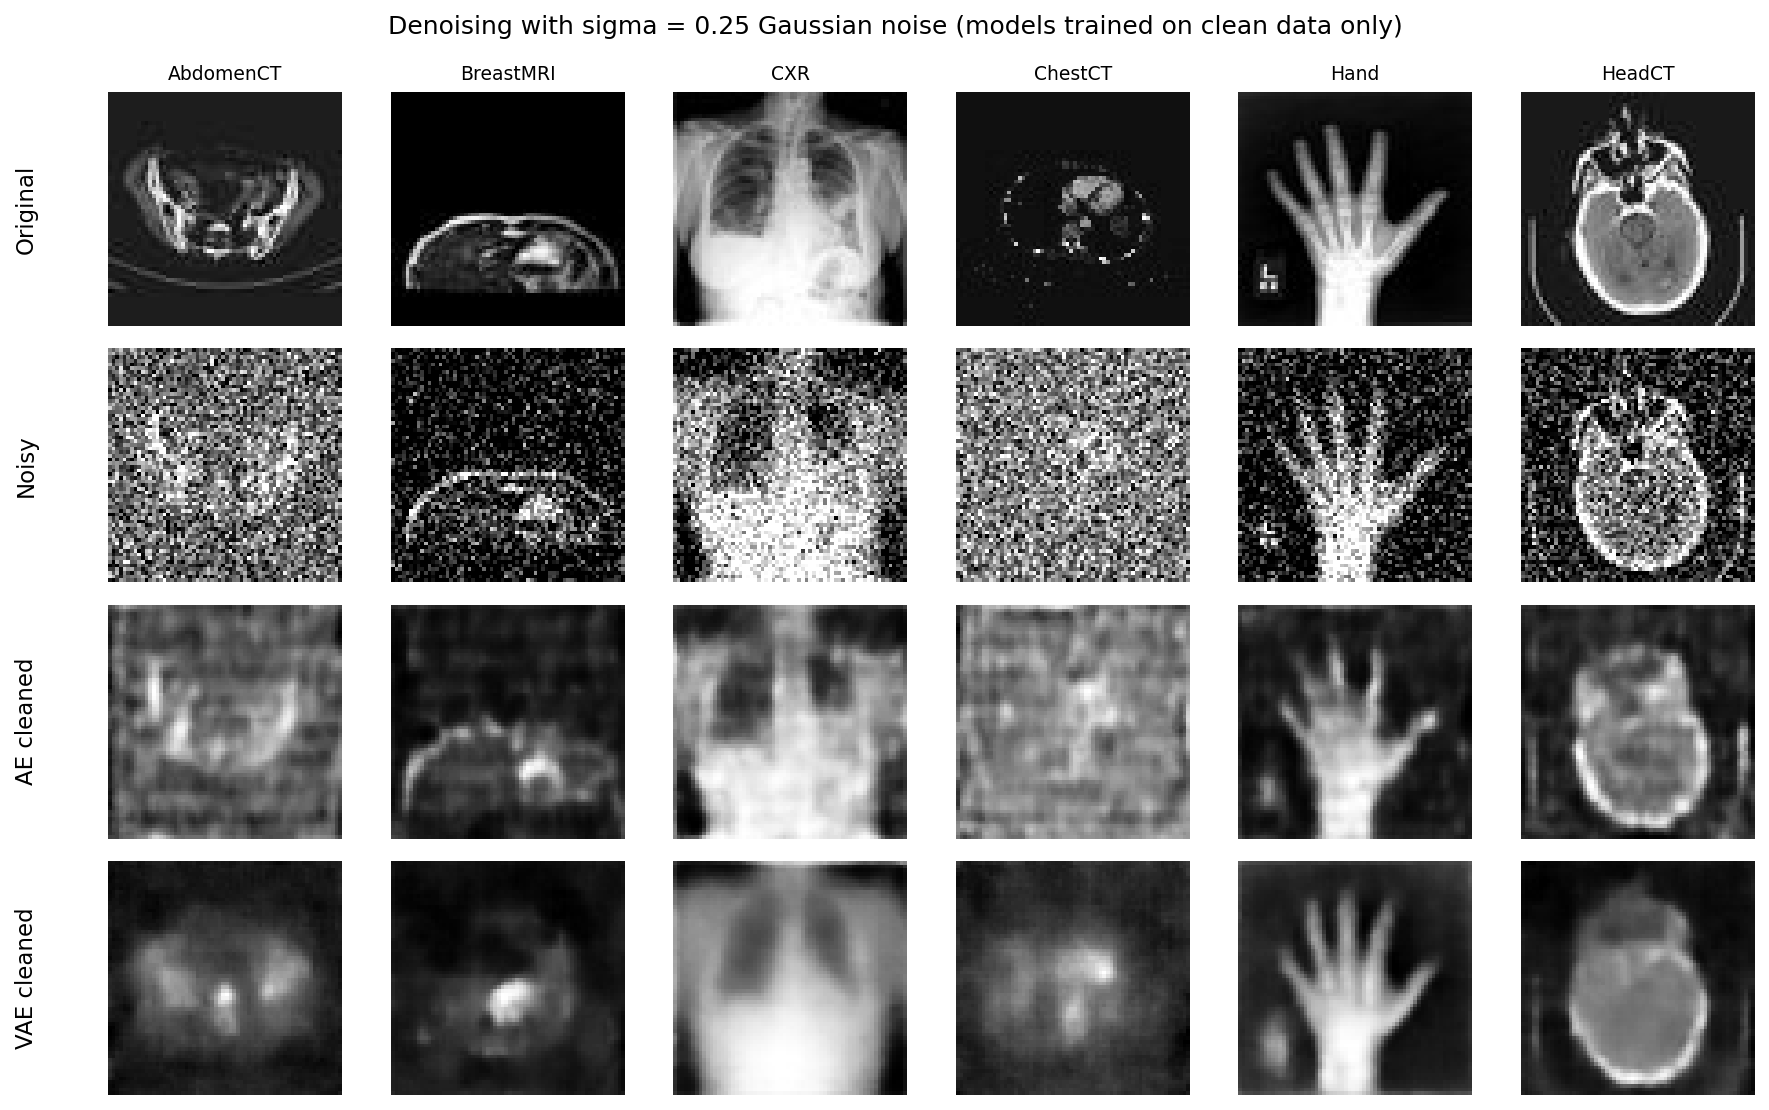
\includegraphics[width=\linewidth]{../figures/08_denoising.png}
  \caption{Both models, trained on clean data only, are fed inputs corrupted with $\sigma{=}0.25$ Gaussian noise. Both suppress most of the noise --- an \emph{emergent} property of the low-dimensional bottleneck. The $\beta$-VAE output is notably cleaner than the AE output, a direct consequence of the prior-regularised latent acting as a stronger implicit smoother.}
  \label{fig:denoise}
\end{figure}

\textbf{Denoising (Fig.~\ref{fig:denoise}).} Although neither model was trained on noisy inputs, both partly denoise $\sigma{=}0.25$ Gaussian corruption because the bottleneck cannot efficiently represent noise. The VAE visibly outperforms the AE here --- an interesting inversion of the reconstruction ranking: the KL-regularised latent acts as a stronger implicit prior against perturbations, whereas the AE's higher-capacity code preserves more of the corruption. A purpose-trained denoising AE with noisy-input / clean-target pairs would outperform both but was out of scope.

\section{Conclusions}
The AE and $\beta$-VAE optimise different objectives and produce different latent geometries. On Medical MNIST, the AE wins on pixel-accurate reconstruction ($39\%$ lower MSE) and on class separability in latent space, making it the better \emph{feature extractor}. The $\beta$-VAE wins on sample generation, latent interpolation, and (unexpectedly) denoising robustness, making it the better \emph{generative model}. Neither model is universally superior; the architectural and loss-function choices encode which downstream capability is prioritised. The $\beta{=}0.25$ weighting was essential to avoid partial posterior collapse; this is a practical tuning point that the canonical $\beta{=}1$ literature tends to understate on small grayscale datasets.

\end{document}
